\subsection{The fixed-volume decision and its objective}
Consider a unit sell order allocated over $N$ execution slots. A feasible schedule belongs to
\[
 \mathcal U=\{u\in\mathbb R^N:u_j\geq0,\ \mathbf1^\top u=1\}.
\]
Here $u_j$ is the fraction sold in slot $j$. Let $L_{jk}=1$ if $k\leq j$ and zero otherwise. The vector $q(u)=\mathbf1-Lu$ measures remaining inventory immediately after each trade; in particular, $q_N=0$. Completion is compulsory, and nonnegative trades exclude buying back inventory during liquidation.

For execution-slot price returns $p$ measured in basis points relative to a fixed decision-time price, define
\begin{equation}
 J_p(u)=K(u)-p^\top u,\qquad
 K(u)=\eta N\|u\|^2+\frac rN\|\mathbf1-Lu\|^2,
 \quad \eta>0,\quad r\geq0.
 \label{eq:objective}
\end{equation}
Higher sale prices reduce this cost. The first term of $K$ is an assumed temporary-impact charge penalising concentrated trading; the second expresses a preference for reducing inventory during execution. The impact--inventory trade-off follows the execution tradition \citep{almgren2001}. In this study neither coefficient is estimated from order-book depth or transaction impact. The inventory term is also not an estimated conditional variance. It is a specified preference within the replay objective.

Because the reference denominator and completed quantity are fixed within an episode, subtracting the same arrival price from every execution price adds only a schedule-independent constant. This permits the use of relative prices in \eqref{eq:objective}. It does not justify changing the denominator between policies. Monetary scoring omits the inventory term while retaining the same schedules, so monetary gain and objective gain answer different questions.

The Hessian of $K$ is
\[
 H=2\eta NI+\frac{2r}{N}L^\top L.
\]
It is positive definite because $\eta>0$. Thus every linear-price perturbation has a unique minimiser on the compact simplex. Write $u_0=\arg\min_{u\in\mathcal U}K(u)$ for the no-signal baseline and $u_1=\arg\min_{u\in\mathcal U}J_\mu(u)$ for the full-exposure schedule induced by a forecast profile $\mu$. The baseline is optimised for the same objective; it need not be a uniform schedule when inventory is penalised.

\subsection{What a terminal forecast leaves unspecified}
\begin{proposition}[Common price-level invariance]
For any scalar $a$, replacing $\mu$ by $\mu+a\mathbf1$ leaves the optimal schedule unchanged. For any two feasible schedules, shifting realised prices by $a\mathbf1$ also leaves their paired objective difference unchanged.
\end{proposition}
\begin{proof}
Every feasible schedule satisfies $\mathbf1^\top u=1$, so
$J_{\mu+a\mathbf1}(u)=J_\mu(u)-a$. The same constant is subtracted for all schedules. For paired realised-price comparisons, $(u-v)^\top\mathbf1=0$ cancels the shift directly.
\end{proof}

The proposition expresses a familiar feature of fixed-volume execution in an elementary finite-grid form. Temporal price contrasts already enter predictive execution models \citep{forde2022,abijaber2025}. The invariance is to a common price level, not to a drift that changes expected prices differently across slots. It also relies on forecast-independent costs and constraints. Price-dependent fees, optional completion, changing impact coefficients or forecast-dependent participation limits require a different comparison.

Knowing $\mu_N$ alone leaves the remaining contrasts unspecified. For a two-slot example, let $K(u)=u_1^2+u_2^2$ and realised prices be $(3,2)$. Forecasts $(2,2)$, $(3,2)$ and $(1,2)$ all predict the terminal price perfectly. Their optimal schedules are respectively $(1/2,1/2)$, $(3/4,1/4)$ and $(1/4,3/4)$. Relative to the flat-forecast baseline, gains are $0$, $0.125$ and $-0.375$. Both nonuniform schedules incur additional cost, but their price alignment has opposite signs. These values are constructed and dimensionless; they are not estimates of crypto execution performance.

The example establishes insufficiency without claiming that an endpoint can never inform timing. A correctly specified parametric path could make all intermediate expectations functions of the endpoint. The diagnostic instead asks what can be concluded when such a path restriction has not been established. Terminal accuracy by itself cannot resolve that missing information.

Figure~\ref{fig:endpoint} illustrates the distinction between a shared terminal prediction and different execution decisions.
\begin{figure}[htbp]
\centering
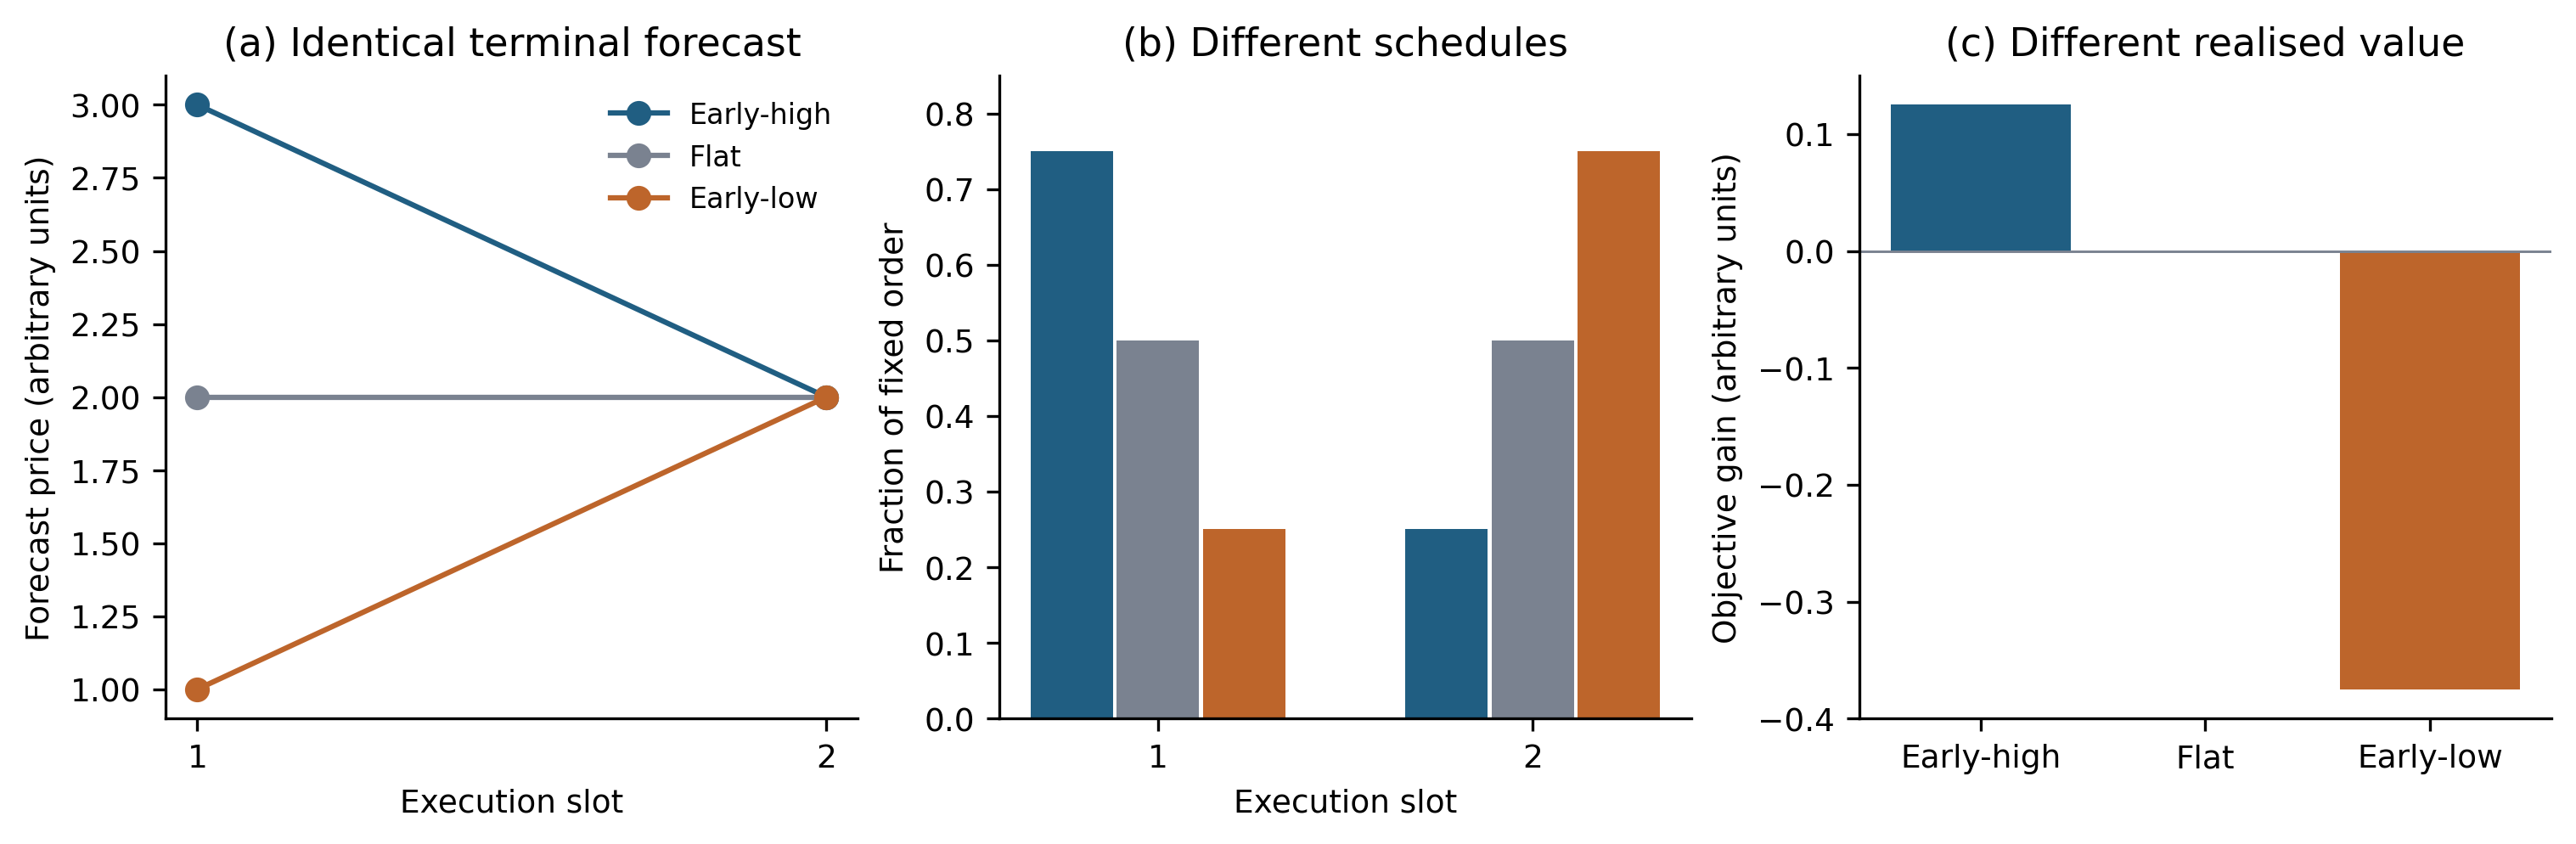
\includegraphics[width=\linewidth]{figures/fig01_endpoint_example.png}
\caption{Synthetic two-slot illustration, not observed market data. The three profiles share terminal forecast 2 but imply different schedules and gains. Prices and objective values are in arbitrary units.}
\label{fig:endpoint}
\end{figure}

\subsection{Exact timing-payoff and action-cost decomposition}
Set $\delta=u_1-u_0$ and mix the feasible schedules as $u(w)=u_0+w\delta$, where $0\leq w\leq1$. Convexity of $\mathcal U$ preserves nonnegativity and completion. The baseline-relative gain is
\begin{equation}
 G(w)=J_p(u_0)-J_p(u(w))=w(A-B)-w^2C,
 \label{eq:gain}
\end{equation}
with
\begin{align}
 A&=\delta^\top p,\qquad
 B=\nabla K(u_0)^\top\delta,\qquad
 C=\tfrac12\delta^\top H\delta.\label{eq:abc}
\end{align}
Equation~\eqref{eq:gain} follows by exact quadratic expansion. Baseline optimality gives $B\geq0$ for a direction toward any other feasible schedule. Also $C>0$ for nonzero $\delta$. If the baseline is interior to the simplex, its gradient is proportional to $\mathbf1$ and $B=0$. The full expression remains valid when constraints bind, so that simplification is not assumed generally.

The price term has a useful inventory interpretation. Define cumulative extra sales $D_j=\sum_{k\leq j}\delta_k$. Completion implies $D_N=0$, and discrete summation by parts gives
\begin{equation}
 A=-\sum_{j=1}^{N-1}D_j(p_{j+1}-p_j).\label{eq:inventory}
\end{equation}
Extra early sales benefit from subsequent declines and lose from subsequent increases. The price movement before the first executable slot cancels because both schedules still hold the full order then. This is exposure accounting, not identification of the hypothetical order's causal market impact.

For any positive exposure, gain is positive precisely when $A-B>wC$. Full exposure requires $A>B+C$. Therefore neither a correct terminal sign nor positive timing alignment alone establishes a worthwhile action. In the quadratic model, the linear payoff falls proportionally with attenuation, whereas curvature cost falls with its square. That relationship explains how a smaller deviation can improve the trade-off. It is conditional on a fixed pair of endpoint schedules; changing the impact coefficient and reoptimising changes the endpoints themselves.

\subsection{Historical exposure fitting}
A common coefficient fitted to historical episodes maximises
$w\overline{(A-B)}-w^2\overline C$. When $\overline C>0$, its solution is
\begin{equation}
 \widehat w_P=\operatorname{clip}_{[0,1]}
 \left\{\frac{\overline{(A-B)}}{2\overline C}\right\}.
 \label{eq:plugin}
\end{equation}
If $\overline C=0$, every direction is zero under the positive-definite Hessian and we select $\widehat w_P=0$. For $C_i>0$, define the realised target $z_i=(A_i-B_i)/(2C_i)$. Then
\[
 G_i(w)=C_i z_i^2-C_i(w-z_i)^2.
\]
Thus historical fitting is equivalent to curvature-weighted squared-error minimisation on the fixed feasible segment. It is not the mean of episode-level ratios, and the realised targets are unavailable at the time the episode's decision is made. Only preceding calibration observations may determine the implemented coefficient.

A lower-percentile variant replaces the historical aggregate ratio with the fifth percentile of day-resampled aggregate ratios before clipping. This is a conservative fitting heuristic, not predictive-coverage calibration or a theorem of safe future improvement. Such distinctions matter because formal decision-focused calibration and conformal coverage refer to different objects and assumptions \citep{liu2021,barber2023}.

Finally, mixing schedules is not generally identical to reoptimising a scaled forecast. With the two-slot cost above and forecast $(6,2)$, the full optimum is $(1,0)$. Half mixing with the baseline gives $(3/4,1/4)$, whereas the endpoint-preserving half-scaled forecast $(4,2)$ still optimises at $(1,0)$. Active-set changes break the global equivalence. Our policies mix the solved schedules, and all reported gains use that operation consistently.
